\section {Обзор инструментов для реализации веб-приложения}

\subsection{Single Page Application}

Основной задачей данного проекта является реализация веб-приложения, взаимодействующее с веб-сервером по протоколу SOAP. Результатом проекта должно получится приложение, которое сможет быстро и мгновенно реализовывать функциональные операции. В настоящее время в сфере веб разработки наряду с многостраничными сайтами (Multi-page Application, MPA) широкое распространение получили и одностраничные приложения (Single-page Application, SPA), формирование контента которых происходит динамически на стороне клиента. В связи с этим было решено реализовывать одностраничное приложение. На рисунках  \ref{mpa} и  \ref{spa} представлена схема работы многостраничного и одностраничного сайта соответственно.

\begin{figure}[ht]
\center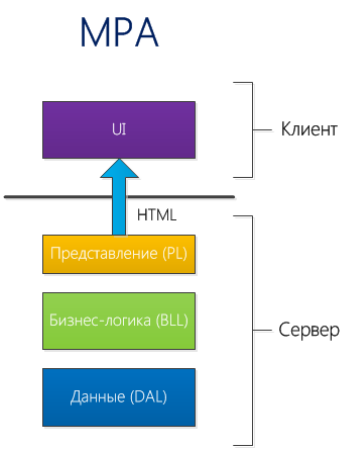
\includegraphics[width=0.4\textwidth]{mpa}
\caption{Архитектура Multi-page Application}\label{mpa}
\end{figure}

\begin{figure}[ht]
\center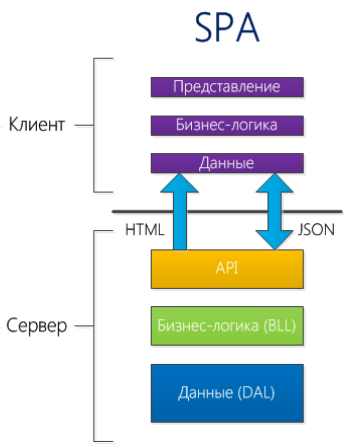
\includegraphics[width=0.4\textwidth]{spa}
\caption{Архитектура Single Page Application}\label{spa}
\end{figure}

Single Page Application -- это веб-приложение, размещенное на одной странице. Применяя такую технологию, можно создать сайт,  который будет представлять собой одну html-страницу, интерактивность которой обеспечивается скриптами. Работа такого веб-сайт максимально полностью перенесена на сторону клиента. Сайт <<общается>> с сервером только чистыми данными, без загрузки html-контента.
 
Для того чтобы написать одностраничное приложение необходимо придерживаться определенных правил:
\begin{enumerate}
\item Все сущности приложения основаны на моделях и объектах. Внутри объектов инкапсулирована работа с DOM-элементами страницы.
\item Насколько позволяет структура хранит HTML шаблоны в скриптах
\item При любые изменения на странице динамически изменяют url.
\item Прямая загрузка любого url должна отобразить соответствующую страницу с данными.
\item Обработчик события History back, что соответствует кнопки назад в браузере, должен выполняться корректно и возвращать страницу в предыдущее состояние.
\item Кеширование моделей данных на стороне клиента.
\end{enumerate}

Если учитывать эти основные правила, в результате получится эффективное, быстрое и полнофункциональное одностраничное веб-приложение.   Но как и любой продукт, приложение обладает рядом преимуществ и недостатков. Рассмотрим плюсы и минусы данного подхода и почему SPA все равно остается популярным.

К преимуществам SPA можно отнести следующее:
\begin{enumerate}
\item Работа на большом количестве устройств. Приложения на SPA отлично работают на устройствах как стационарных, так и мобильных. Персональные компьютеры, планшеты, смартфоны могут беспрепятственно работать с сайтами построенных по принципу SPA. Создав одно приложение, мы получим гораздо большую аудиторию пользователей нежели при использовании стандартного подхода.
\item  Богатый пользовательский интерфейс. Так как веб-страница одна, построить функциональный и приятный пользовательский интерфейс гораздо проще. Не так затруднительно хранить информацию о сеансе, управлять состояниями представлений и управлять анимацией.
\item Отсутствие загрузки одного и того же контента снова и снова. Если сайт использует шаблон, то вместе с основным содержанием какой-либо страницы посетитель сайта обязательно загружает разметку шаблона. Конечно, кеширование данных на данном этапе развития в веб-программировании достигло высоких результатов, но если нечего кешировать, то время  и ресурсы на это не тратятся.
\end{enumerate}

Самым главным неудобством при разработке SPA -- это работа с языком программирования JavaScript. JavaScript изначально позиционировался как простой язык программирования с Java-подобным синтасисом. Но  JavaScript не обладает статической типизацией, его объектная модель не является привычной для многих разработчиков. Отладка кода представляет собой трудный процесс. Кроме того, различные интернет-обозреватели могут по-разному интерпретировать JavaScript-код. Поэтому разработка требуемого приложения с использованием исключительно языка JavaScript является довольно трудоёмким процессом. Чтобы как-то исправить несовместимость с некоторым браузерами, приходится писать отдельный код для различных клиентов. Таким образом, размер кода возрастает, а функциональность нет. В итоге приходится основную часть времени тратить на обработку особенностей выполнения кода различными движками, а не на реализацию продукта. Частично последнюю проблему можно решить использованием специальных библиотек, примеру, библиотека jQuery.  


\subsection {JavaScript-фреймворки}

На смену библиотекам вроде jQuery в мир JavaScript приходят фреймворки, реализующие функциональную схему Model-view-controller. 

Model-view-controller (MVC) -- схема использования нескольких шаблонов проектирования, с помощью которых модель приложения, пользовательский интерфейс и взаимодействие с пользователем разделены на три отдельных компонента таким образом, чтобы модификация одного из компонентов оказывала минимальное воздействие на остальные. Архитектура работы MVC представлена на рисунке \ref{mvc}

\begin{figure}[ht]

\center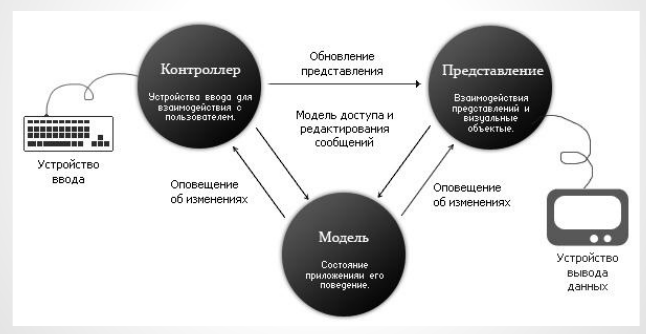
\includegraphics[width=0.7\textwidth]{mvc}

\caption{Схема Model-view-controller}\label{mvc}

\end{figure}

Концепция MVC позволяет разделить данные, представление и обработку действий пользователя на три отдельных компонента:
\begin{enumerate}
\item Модель (англ. Model). Модель предоставляет знания: данные и методы работы с этими данными, реагирует на запросы, изменяя своё состояние. Не содержит информации, как эти знания можно визуализировать.
\item Представление, вид (англ. View). Отвечает за отображение информации (визуализацию). Часто в качестве представления выступает форма (окно) с графическими элементами.
\item Контроллер (англ. Controller). Обеспечивает связь между пользователем и системой: контролирует ввод данных пользователем и использует модель и представление для реализации необходимой реакции.
\end{enumerate}

Важно отметить, что как {\itshape представление}, так и {\itshape контроллер} зависят от {\itshape модели}. Однако модель не зависит ни от представления, ни от контроллера. Тем самым достигается назначение такого разделения: оно позволяет строить модель независимо от визуального представления, а также создавать несколько различных представлений для одной модели.


Преимущества фреймворков видны невооруженным глазом. Один из самых существенных является избавление от рутинного кода, который тянется от проекта к проекту. Фреймворк предоставляет разработчикам каркас будущего приложения и решение задач, встречающихся в большинстве проектов. Например, программисту не нужно думать, как принять данные от клиента и передать их на сервер, т.к. все необходимое скорей всего реализовано авторами фреймворка. Вместо этого разработчику предлагается сосредоточиться функционалом собственного приложения.

Другим немаловажным плюсом всех фреймворков является стандартизация кодирования. Если разработчик решается применять готовый каркас в своем проекте, то он должен быть готовым следовать его заповедям. Это значит, что ему нужно не полениться - один раз ознакомиться с правилами и быть спокойным, что в последствие код без проблем может дорабатываться другими разработчиками. 

Очень часто многие разработчики задают вопрос -  Чем один Javascript фреймворк лучше другого? На этот вопрос трудно ответить, ведь каждый фреймворк обладает определенным набором инструментов и имеет свой круг задач, с которыми он успешно справляется. Выбор JavaScript MVC фреймворка — тяжёлая работа. Нужно учесть много факторов, и число вариантов выбора может быть огромно. 


Для создание приложения на основе SPA необходимо отобрать несколько фреймворков, чей функционал справится с поставленной задачей, рассмотреть сильные и слабые стороны каждого и выбрать подходящий вариант.

\subsection {Angular}

AngularJS --- MVW-фреймворк для разработки качественных клиентских веб-приложений на JavaScript. Он создан и поддерживается в Google и предлагает взглянуть на будущее веба, на то, какие новые возможности и стандарты он готовит для нас. MVW означает Model-View-Whatever (модель--вид--что-угодно), то есть гибкость в выборе шаблонов проектирования при разработке приложений. Мы можем выбрать модели MVC (Model--View--Controller) или MVVM (Model--View--View--Model) [4].

AngularJS является основой, которая связывает HTML-код, который генерируется для просмотра страницы в окне браузера с JavaScript объектами. Когда изменяется один из объектов, автоматически обновляется и генерируемая страница. Верно и обратное --- модели связаны с контентом страницы. Когда изменяется контент, это вызывает изменения и в коде сайта. Это называется двусторонней связью данных, схематично представленной на рисунке \ref{dual}.

\begin{figure}[ht]
\center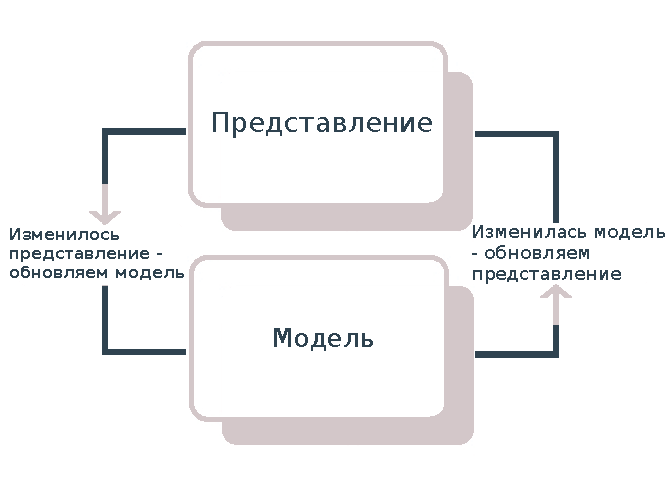
\includegraphics[width=0.9\textwidth]{dual}
\caption{Схема двусторонней привязки данных}\label{dual}
\end{figure}

AngularJS связывает коды в единую систему, и разработчику не нужно больше обновлять HTML вручную или инспектировать элементы, как в случае, если приходится использовать JQuery.
Инъекция зависимостей – шаблон разработки программ, который определяет, как компоненты связываются со своими зависимостями. Инъекция — это передача зависимости к зависимому Объекту, и эти зависимости часто называют Сервисами.

В AngularJS используются аргументы функции для объявления нужных зависимостей. Если мы забудем передать зависимость, но сошлёмся на неё там, где она нужна нам, Сервис будет не определен и в результате произойдёт ошибка компиляции внутри Angular. Однако, Angular выбрасывает свои ошибки, и они очень просты в отладке.

Одно из основных понятий в программировании – область видимости. В Angular область видимости – это один из главных объектов, который делает возможным циклы двусторонней связи данных и сохраняет состояние приложения. \textdollar scope --- объект, который не только имеет доступ к данным и значениям, но и предоставляет эти данные в DOM, когда Angular рендерит наше приложение.

\textdollar scope – это автоматический мост между JavaScript и DOM, хранящий синхронизированные данные[4]. Это позволяет проще работать с шаблонами, когда мы используем при этом синтакс HTML, а Angular рендерит соответствующие значения \textdollar scope. Это создаёт связь между JavaScript и DOM. Таким образом, \textdollar scope играет роль ViewModel.

Контроллер позволяет взаимодействовать Виду и Модели. Это то место, где логика презентации синхронизирует интерфейс с моделью. Цель Контроллера – приводить в действие изменения в Модели и Виде. В Контроллере Angular сводит вместе бизнес-логику и логику презентации. Контроллер принимает два аргумента – имя, по которому на него можно ссылаться, и функцию обратного вызова. При этом на самом деле это будет функция, описывающая тело Контроллера.

Цель Контроллера – интерпретировать бизнес-логику модели и преобразовывать её в формат презентации. В AngularJS это можно делать по-разному, в зависимости от того, какие мы получаем данные.
Контроллер общается с Сервисом, и передаёт данные в том же, или изменённом формате в наш Вид через объект \textdollar scope. Когда Вид обновлён, логика Контроллера также обновляется, и её можно передавать обратно на сервер через Сервис.
HTML отлично подходит для описания статичных документов, но теряет свою эффективность при попытке описать динамические виды в веб-приложениях. AngularJS позволяет расширить синтаксис HTML. В результате код получается выразительным, читаемым, и легко поддерживается.

\subsection {BackBone}

Приложения на Backbone не придерживаются строгой архитектуры. Основная идея, которую несёт документация: используйте инструменты этого фреймворка так, как вам хочется. Благодаря такому подходу Backbone хорош для абсолютно разных задач, и на нем очень просто начать писать приложения. Однако с другой стороны, это приводит к тому, что новички совершают ошибки в самом начале работы с ним. 

Работая с Backbone, данные представляются как Модели (Models), которые могут быть созданы, провалидированы, удалены, и сохранены на сервере. Всякий раз, когда в интерфейсе изменяется атрибуты модели, модель вызывает событие "change"; все Представления (Views), которые отображают состояние модели, могут быть уведомлены об изменении атрибутов модели, с тем чтобы они могли отреагировать соответствующим образом — например, перерисовать себя с учетом новых данных. При изменении модели представление просто обновит себя самостоятельно.

Рассмотрим поподробней сущности Backbone, их предназначение и минимальную реализацию:
\begin{enumerate}
\item Backbone.Model; Model  -- это единица данных. Отвечает за получение, отправку, хранение, валидацию и прочие манипуляции с данными какой-то сущности. Простая реализация такой единицы данных представлена на рисунке \ref{modal}.

\item Backbone.Collection; Collection -- это упорядоченный набор  моделей. Отвечает за получение и отправку данных какой-то сущности, а так же манипуляции с моделями (создание, обновление, удаление). Работает только с моделями определенного типа. Простая реализация такого списка представлена на рисунке \ref{collection}.

\item Backbone.View; View -- это представление модели или коллекций, отвечает за реализацию интерфейса. Отвечает за рендеринг модели или коллекции, работу с шаблонами, обработку событий и другое. Простая реализация представлена на рисунке \ref{view}.

\item Backbone.Router; Router предоставляет методы для маршрутизации на стороне клиента, а также связывания этих действий с событиями. Простая реализация таких методов представлена на рисунке \ref{router}.

\end{enumerate}

\begin{figure}[ht]
\center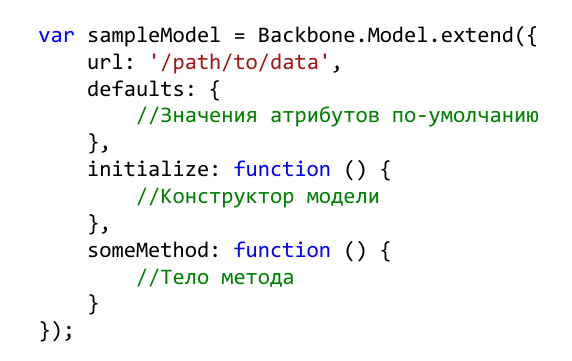
\includegraphics[width=0.75\textwidth]{model}
\caption{Backbone.Model}\label{modal}
\end{figure}

\begin{figure}[ht]
\center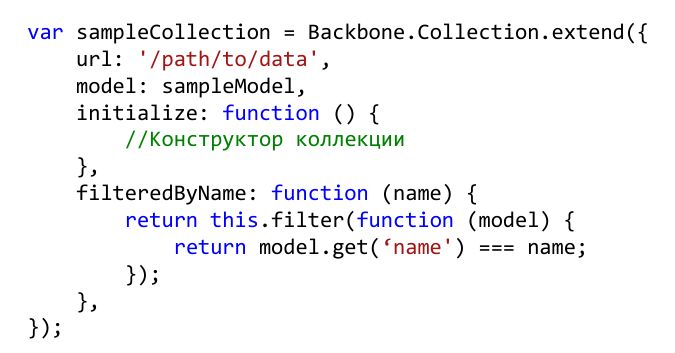
\includegraphics[width=0.75\textwidth]{collection}
\caption{Backbone.Collection}\label{collection}
\end{figure}


\begin{figure}[ht]
\center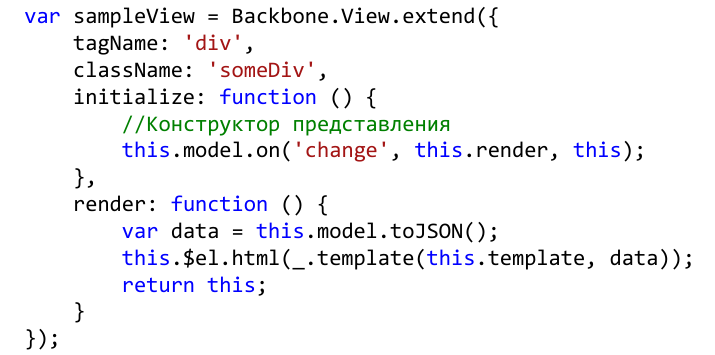
\includegraphics[width=0.75\textwidth]{view}
\caption{Backbone.View}\label{view}
\end{figure}

\begin{figure}[ht]
\center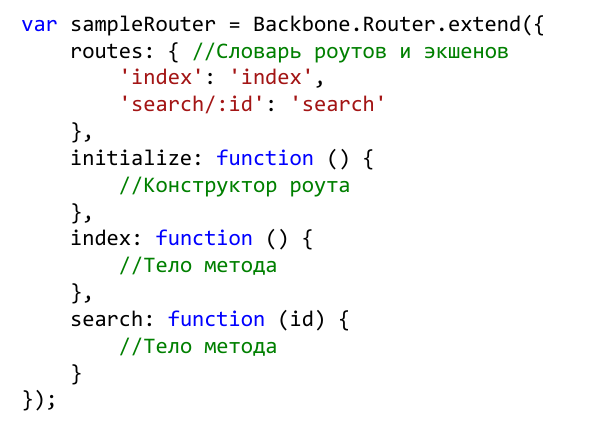
\includegraphics[width=0.75\textwidth]{router}
\caption{Backbone.Router}\label{router}
\end{figure}

\subsection {Сравнение Angular и BackBone}

Перед тем как реализовывать приложение, были тщательно изучены и опробованы оба фреймворка. Были выбраны характеристики, которые являются важными при реализации приложения, и на основе полученных данных произвели сравнение фреймворков. характеристики для сравнения:
\begin {enumerate}
\item Порог входа и документация
\item Продуктивность разработки
\item Набор функций
\item Размер 
\item Защита от утечки памяти 
\end {enumerate}

{\itshape Порог входа и документация}

Angular легко позволяет делать сложные вещи такие, как двунаправленная синхронизация. Но после освоения базовых знаний, порог обучения становится выше: открывается сложная структура с большим количеством особенностей. Чтение документации затруднено из-за специфического жаргона и малого количества примеров.

Backbone — довольно прост в освоении. Но после длительного использования вы можете обнаружить, что не хватает понимания того, как лучше структурировать код. Чтобы исправить сложившуюся ситуацию необходимо просмотреть или прочитать несколько учебников. 

{\itshape Продуктивность разработки}

Разработка с помощью Angular будет достаточно быстрой и эффективной, после того, как изучить его основные функции и принцип работы.

Backbone требует написания очень большого объёма шаблонного кода. Что оказывается прямой угрозой производительности труда и является неэффективным.

{\itshape Набор функций}

Среди основного набора функций, которым обладает схема MVC является:
\begin{enumerate}
\item Реализация паттерна <<Наблюдатель>>: объекты, изменения которых отслеживаются.
\item  Наличие автоматически изменяемых представлений
\item Представления (визуализация шаблонов), включающие другие представления.
\item Показ представлений по некоторым условиям.
\item Использование автоматически изменяемых представлений, когда наблюдаемый объект изменяется.
\end{enumerate}

Angular полный набор перечисленных функций.

Backbone, в свою очередь, иметь только реализацию паттерна <<Наблюдатель>>

{\itshape Размер и зависимости} 

Является важным фактором для мобильной разработки.

Angular имеет размер в 80 килобайт, однако это единственный фреймворк, не требующий дополнительных библиотек.

Backbone считается самым маленький фреймворк, но требует как минимум две библиотеки, что увеличивает размер фреймворка до 61 килобайта.

{\itshape Защита от утечки памяти} 

Так же является важным фактором для длительно открытых одностраничных приложений.

С фреймворком Angular можно эффективно решать проблему с утечкой памяти, даже не обладая огромным опытом в разработке.

Что нельзя сказать о фреймворке Backbone. При недостаточных знаний эта проблема окажется глобальной.

\subsection{Apache Cordova}
На сегодняшний день люди везде используют мобильные устройства для самых различных потребностей. Будь то фотографирование и размещения снимков в социальных сетях, поиска местоположения ресторана или просмотра заголовков новостей. Мобильные устройства имеют множество форм и стилей. Мобильные телефоны работают на разных операционных системах, таких как Apple iOS, Google Android и Research In Motion Blackberry. Некоторые имеют большие экраны, физические клавиатуры и работают в сетях 3G, 4G или WiFi. Мобильные телефоны могут также иметь датчики ускорения, местоположения и даже платежей. Некоторые из этих устройств - даже не телефоны; это планшеты с более крупными экранами и сетевым подключением только для обмена данными.

Несмотря на различия, мобильные устройства похожи друг на друга тем, что все они исполняют мобильные приложения. Мобильные приложения можно разделить на три типа: встроенные, веб-приложения и гибридные.

Установленные на устройство встроенные приложения представляют собой бинарные исполняемые программы, созданные с использованием соответствующего  SDK  и  распространяемые  через  хранилища приложений. SDK существуют для каждой мобильной операционной системы и, конечно же, различаются между собой.

В отличие от встроенных веб-приложения загружаются в мобильный веб-браузер, их код пишется с использованием веб-технологий (HTML, JavaScript и CSS), не зависящих от операционной системы устройства. Нет необходимости изучать различные языки программирования для каждого устройства. HTML и JavaScript знакомы веб-разработчикам по созданию веб-страниц для настольных браузеров. В большинстве случаев мобильные веб-браузеры могут визуализировать те же самые веб-страницы, но веб-сайты часто предоставляют мобильные версии с меньшим объемом информации и более быстрой загрузкой (из-за меньшего размера экрана и более медленной сети).

Для запуска веб-приложения пользователь вводит URL-адрес в мобильный веб-браузер. После этого загружается веб-страница, являющаяся точкой входа в веб-приложение. Веб-приложения не распространяются через хранилище приложений; они являются обычными ссылками, которые можно включить в другие веб-страницы.

Гибридные приложения, как и веб-приложения, программируются с использованием веб-технологий, но пакетируются как встроенные приложения. Гибридное приложение можно написать сразу для нескольких мобильных операционных систем с использованием языка программирования, знакомого многим разработчикам. Поскольку гибридное приложение на самом деле является встроенным, вы получаете доступ к функциям устройства из JavaScript, что пока недоступно для веб-приложений.

Гибридные приложения можно распространять и устанавливать через хранилища приложений, подобно встроенным. Apache Cordova позволяет создавать универсальные мобильные приложения, работающие на различных мобильных платформах, с использованием стандартных веб-технологий (HTML5, CSS3 и JavaScript), что отабражено на рисуноке \ref{cordova}.

\begin{figure}[ht]
\center
\includegraphics[width=0.9\textwidth]{cordova}
\caption{Apache Cordova}\label{cordova}
\end{figure}

Использование Apache Cordova в качестве базового фреймворка, позволяет создавать приложения, функционирующие на широком спектре мобильных платформ, включая Tizen, webOS, Android, iOS, Blackberry, Samsung Bada и Windows Phone\cite{cordova}.

Cordova предоставляет среду для хостинга контента HTML5/JavaScript внутри тонкой <<родной>> оболочки. Для ОС на каждой платформе смартфонов она использует родной элемент управления <<браузер>> для рендеринга контента создаваемого приложения, причем ресурсы приложения упаковываются в дистрибутив.

Cordova также предоставляет набор стандартных API для доступа к функциям, общим для всех смартфонов. К некоторым из этих функций относятся:
\begin{enumerate}
\item События жизненного цикла приложения.
\item Хранилище (локальное хранилище и базы данных HTML5).
\item Контакты.
\item Камера.
\item Геопозиционирование.
\item Акселерометр.
\end{enumerate}
Каждая из этих функций предоставляется как JavaScript API, который используется из кода на JavaScript. Cordova берет на себя всю черновую работу, связанную с предоставлением необходимой родной реализации, и тем самым гарантирует, что программист будет иметь дело с одинаковыми JavaScript API независимо от ОС смартфона, на котором выполняется код создаваемого приложения. 

